\documentclass{article}

\usepackage{polski}
\usepackage{geometry}
\usepackage[utf8]{inputenc}
\usepackage{amsmath}
\usepackage{algorithm}
\usepackage{algorithmic}
\usepackage{graphicx}
\graphicspath{ {/home/konrad/Semestr5/Semester-5/ObliczeniaNaukowe/lab3/src} }
\geometry{
	a4paper,
	total={170mm,257mm},
	left=20mm,
	top=20mm,
}

\begin{document}
		\title{Obliczenia naukowe, lista nr 5}
	\author{Bartosz Banasik}
	\maketitle
	
	\pagenumbering{arabic}
	
	\section{Zadanie 1}
	\paragraph{Polecenie:}
	Napisać algorytm rozwiązujący układ liniowych równań $Ax = b$ metodą eliminacji Gaussa uwzględniając przy tym specyficzną postać macierzy, która jest odpowiednio gęsta na przekątnej.
	\subsection{Rozwiązanie}
	 Aby móc rozwiązać około $50000$ równań liniowych potrzebna jest odpowiednia struktura, która będzie pamiętać tylko elementy niezerowe. Julia dostarcza nam takich narzędzi. (sparse matrix) Kolejnym problemem jest czas obliczeń. Pospolita eliminacja Gaussa ma złożoność $O(n^3)$, jednak mając specyficzną postać macierzy do rozwiązania jesteśmy w stanie ją zmniejszyć. Zauważmy, że podczas zerowania kolejnych komórek wierszy nie musimy robić tego na całej wysokości macierzy. Wystarczy że ograniczymy się do wartości które, mogą nie być zerowe. Podobnie jest ze zmianą wartości w wierszu. Nie musimy zmieniać całego wiersza, tylko komórki odpowiednio blisko przekątnej. Stosując te optymalizacje, wszystkie obliczenia będą się wykonywać na przekątnej i nie będą znacznie odbiegały od niej na więcej niż $l$.  Eliminacja Gaussa z częściowym wyborem elementu głównego polega dodatkowo na sprawdzeniu czy w którejś komórce pod przekątną, dla której wykonywane jest zerowanie, ma większą wartość bezwzględną niż aktualna przekątna.
	\subsection{Wyniki}
	
	Przykładowy wynik dla danych testowych:\newline
		\begin{center}
			\begin{tabular}{|r|r|}
				$x[1]$ & 1	\\
				$x[2]$ & 1	\\
				$x[3]$ & 1	\\
				... & ... \\
				$x[15]$ & 1	\\
				$x[16]$ & 1	\\
			\end{tabular}
		\end{center}
	Przykładowe czasy dla rozmiarów macierzy:
	\begin{center}
		\begin{tabular}{|c|c|}
			rozmiar & czas \\
			400 & 0.00069\\
			10000 & 0.272655661\\
			50000 & 7.676598031\\
		\end{tabular}
	\end{center}
	Dla metody eliminacji Gaussa z częściowym wyborem elementu głównego:
	\begin{center}
	\begin{tabular}{|c|c|}
		rozmiar & czas \\
		400 & 0.001887008\\
		10000 & 0.418363167\\
		50000 & 10.725192563\\
	\end{tabular}
\end{center}	

	\paragraph{Wykresy}
	Poniżej znajdują się wykresy wygenerowane dla wyżej opisanych algorytmów.
	\begin{figure}[H]
		\centering
		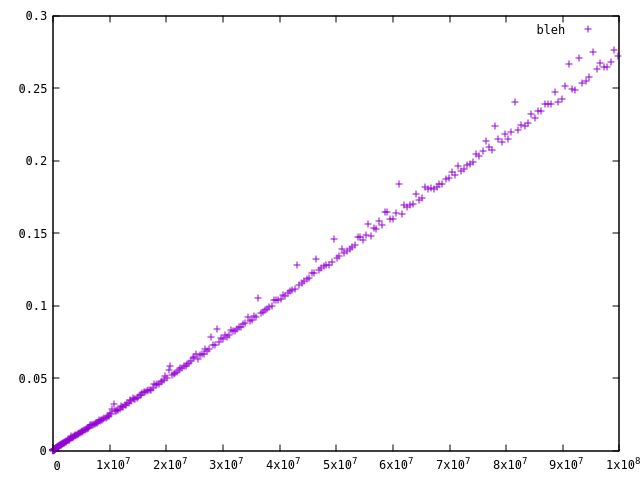
\includegraphics[width=0.6\linewidth]{wykres.png}
		\caption{Wykres czasu do pola tablicy.}		
	\end{figure}
	\begin{figure}[H]
	\centering
	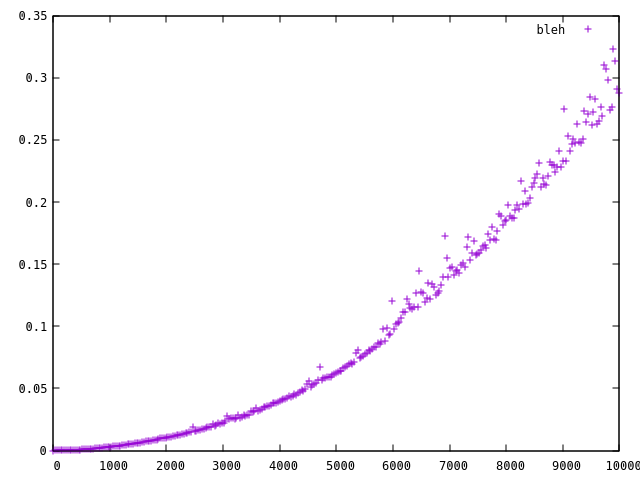
\includegraphics[width=0.6\linewidth]{wykres1.png}
	\caption{Wykres czasu do szerokości tablicy.}		
\end{figure}

	\begin{figure}[H]
	\centering
	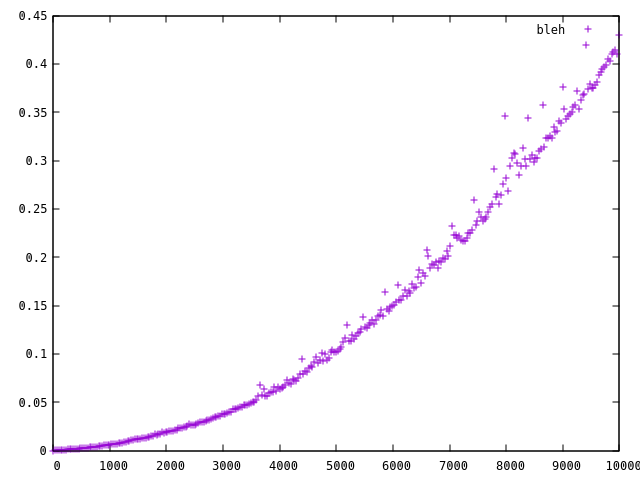
\includegraphics[width=0.6\linewidth]{wykres3.png}
	\caption{Wykres czasu do szerokości tablicy (z wyborem).}		
\end{figure}

	\paragraph{Wnioski:}
Zaproponowany algorytm pozwala efektywnie obliczyć rozwiązania zadanego układu, nawet dla bardzo dużej ilości danych. Oraz pokazuje, że zmniejszyliśmy złożoność obliczeniową.
	\end{document}